% THIS IS SIGPROC-SP.TEX - VERSION 3.1
% WORKS WITH V3.2SP OF ACM_PROC_ARTICLE-SP.CLS
% APRIL 2009
%
% It is an example file showing how to use the 'acm_proc_article-sp.cls' V3.2SP
% LaTeX2e document class file for Conference Proceedings submissions.
% ----------------------------------------------------------------------------------------------------------------
% This .tex file (and associated .cls V3.2SP) *DOES NOT* produce:
%       1) The Permission Statement
%       2) The Conference (location) Info information
%       3) The Copyright Line with ACM data
%       4) Page numbering
% ---------------------------------------------------------------------------------------------------------------
% It is an example which *does* use the .bib file (from which the .bbl file
% is produced).
% REMEMBER HOWEVER: After having produced the .bbl file,
% and prior to final submission,
% you need to 'insert'  your .bbl file into your source .tex file so as to provide
% ONE 'self-contained' source file.
%
% Questions regarding SIGS should be sent to
% Adrienne Griscti ---> griscti@acm.org
%
% Questions/suggestions regarding the guidelines, .tex and .cls files, etc. to
% Gerald Murray ---> murray@hq.acm.org
%
% For tracking purposes - this is V3.1SP - APRIL 2009

\documentclass{acm_proc_article-sp}

\begin{document}

\title{Prototype of an event-driven Future Internet Cockpit -  Real-Time Sensor Events for Complex Event Processing}
% \subtitle{[Event processing]}

%
% You need the command \numberofauthors to handle the 'placement
% and alignment' of the authors beneath the title.
%
% For aesthetic reasons, we recommend 'three authors at a time'
% i.e. three 'name/affiliation blocks' be placed beneath the title.
%
% NOTE: You are NOT restricted in how many 'rows' of
% "name/affiliations" may appear. We just ask that you restrict
% the number of 'columns' to three.
%
% Because of the available 'opening page real-estate'
% we ask you to refrain from putting more than six authors
% (two rows with three columns) beneath the article title.
% More than six makes the first-page appear very cluttered indeed.
%
% Use the \alignauthor commands to handle the names
% and affiliations for an 'aesthetic maximum' of six authors.
% Add names, affiliations, addresses for
% the seventh etc. author(s) as the argument for the
% \additionalauthors command.
% These 'additional authors' will be output/set for you
% without further effort on your part as the last section in
% the body of your article BEFORE References or any Appendices.

\numberofauthors{1} %  in this sample file, there are a *total*
% of EIGHT authors. SIX appear on the 'first-page' (for formatting
% reasons) and the remaining two appear in the \additionalauthors section.
%
\author{
% You can go ahead and credit any number of authors here,
% e.g. one 'row of three' or two rows (consisting of one row of three
% and a second row of one, two or three).
%
% The command \alignauthor (no curly braces needed) should
% precede each author name, affiliation/snail-mail address and
% e-mail address. Additionally, tag each line of
% affiliation/address with \affaddr, and tag the
% e-mail address with \email.
%
% 1st. author
\alignauthor
Robin B\"ohm\\
       \affaddr{University of Duisburg Essen}\\
       \affaddr{paluno - The Ruhr Institute for Software Technology}\\
       \affaddr{Sch\"utzenbahn 70, 45117, Essen, Germany}\\
       \email{robin.boehm@stud.uni-due.de}
}

\maketitle
\begin{abstract}

In this project we developed a prototype for an architecture for an event-driven cockpit in the Future Internet(FI) context.
The prototype is about monitoring a business case of perishable goods in the logistic domain to improve the reaction time issues through the combination of some state-of-the-art technologies.

It uses a service platform that provides sensor event data for things in the real-wold that are provided via the websocket protocol - this platform based on the Internet of Things (IoT) concept. 
These events are aggregated and interpreted by an Complex Event Engine(CEP) and visualized via an HTML5 cockpit in a web-browser.
Through the chosen architecture the latency between the actual business event and the visualization is nearly real-time.
\end{abstract}


\section{Introduction}
The aim of this project is to combine some of the state-of-the-art Future Internet(FI) technologies and using them to implement a prototype for a specific use-case that bring out the advantages of such a system.
The chosen use-case is a business process management in the logistic sector that handles with perishable goods. To manage this task it is necessary to manage trucks, routes and have an overview about the current state of the deliveries. We focused on the reducing of the latency between the actual business event and the delivery of the information to improve the possibility to react quickly to this events and increase the value of this information as shown by Hackathorn\cite{hackathron:real_time_to_real_value}.

We are using the Internet of Things(IoT) and Internet of Services(IoS) concepts to linking the real-world with our business world. So we are able to use real-time sensor events to create our virtual model. We are able increase the amount and quality of event-data that can be used for calculations and combine them to more valuable complex events.
To handle the messaging inside of our prototype we decided to use an Event-driven-Architecture(EDA) in combination with an Complex-Event-Processing(CEP) Engine to defining the rules for our complex events.

We are providing a cockpit for monitoring the business model with some useful visualizations.This cockpit is implemented with modern web technologies so it is usable on many devices out of the box over the specifications. It contains a map that shows the current state of given routes with an rating calculated on the raw events. Also a table that offers information in more textual way.

This paper starts with an introduction about the basics in section \ref{sec:Basics}.
After a survey of related work in Section \ref{sec:Related Work}. 
The Use-Case is described in section \ref{sec:Use Case} and our design considerations of the different components are part of section \ref{sec:Conceptional Design}.
The next section \ref{sec:Implementation} contains details about the implementation with a technical stack component overview followed by the conclusion in section \ref{sec:Conclusion}.

\section{Basic}
\label{sec:Basics}

The idea of \textbf{Future Internet} is to enhance the architectures for the current state of the Internet. There are many ideas that are elaborated and discussed. The \textbf{Internet-of-Things} term first used by Kevin Ashton in the year 1999 \cite{•}. He describes the IoT as enhancement from human-entered data to real world data that is captured by machines.
\begin{quote}
If we had computers that knew everything there was to know about things - using data they gathered without any help from us - we would be able to track and count everything, and greatly reduce waste, loss and cost. We would know when things needed replacing, repairing or recalling, and whether they were fresh or past their best. 
\end{quote}
That is a quote from an article he published 2009 in the RFIDJournal
\cite{iot_thing:Ashton}.
There is another concept of FI that could enables us to use all this information that is called \textbf{Internet of Services}. This is a concept that describes next-generation services that are world-wide available and could be used. They are highly adaptive and can be integrated in own services \cite{future_Internet:shenker}.
A service platform that is named COSM and described itself as `Internet of Things Platform' on the website\cite{cosm} is implementing this kind of idea. This platform enables developers and companies to connect devices and exchange data over an defined API that use the websocket protocol.

The websocket protocol is an http upgrade protocol that enables a two-way communication between a client and a remote host \cite{websocket}. It was developed to provide a mechanism for browser-based applications that need this kind of communication wihout relying on multiple HTTP connections e.g. long polling\cite{long_polling}. 

To handle this high amount of realt-time data in information systems is likely to use an \textbf{event-driven-architecture} (EDA). An EDA is defined as one that has the ability to detect events and react intelligently on them. Also its designed to handle real-time or nearly real-time changes in business conditions.\cite{EDA:Taylor}

To add some more more meaningful value for some special business case\textbf{Complex Event Processing}(CEP) can be used. CEP is a method that tracks and analyses events and combine them to more valuable complex events. A complex event can be defined through rules and combined, integrate or aggregate other events. Also temporal rules can be defined that detecting the occurrence of events in a defined time interval.

\section{Related Work}
\label{sec:Related Work}

TODO!!

\section{Use Case}
\label{sec:Use Case}

Basically our use case is about managing the delivery of perishable goods. This is a high risk business process in the logistic domain. If some goods arriving late or there are some problems with the cooling system it is necessary to get the information of the real-world state as quick as possible to do a trade-off what could be the best action to reduce risk or costs.

Our scenario comprises the planing and alternatives in escalation situations of the delivery of these perishable goods via trucks over a defined route. These trucks are equipped with sensors that provides us the monitoring data that is used for automated real-time aggregation and interpretation and share the results in a cockpit application like it is described in the Internet-of-Things(IoT) concept. 
Also the routes are equipped with sensors that enables us to monitor them.
The overview in such a business monitoring tool is modeled a cockpit with summary of meaningful information that should support the decision. 

The cockpit provides an ampel-system with the colors green,yellow and red that visualizing the current state of the routes and trucks depending on defined threshold.
Also the prototype is using complex threshold for combinations of singular states of a route or a truck that currently on this route that are also visualized in a map.
The cockpit should be available via different devices like on the computer or on smart-phone.
%Actuality of the information is one of the most valuable criterion
\section{Conceptional Design}
\label{sec:Conceptional Design}

As basic architectural design we are choosing to build an event-driven-architecture(EDA).
An EDA is loosely coupled and can be used for distribution and scalability of software components. Because every component could have multiple listeners for his own events or act as sender for multiple other components.
For our prototype we build service components that are loosed coupled and communicating only via events.
At first we using a connector that receives basic events from the COSM Service API.
The component connects to the API and subscribe itself to the relevant data-streams that are prepared for this demo-case.
Once the component is registered to the service-api, it receives an event via push every time a change of state appears at the data-stream. Through the static connection that happens in real-time without any overhead to create a new TCP HTTP connection.
When the event message is arrived via the socket it get parsed and transformed into the internal event structure and directly send to the components that are listening.
A registered listener in our system for this COSM-Component Events is the Complex-Event-Processing(CEP) component.

\begin{figure}
	\begin{center}
		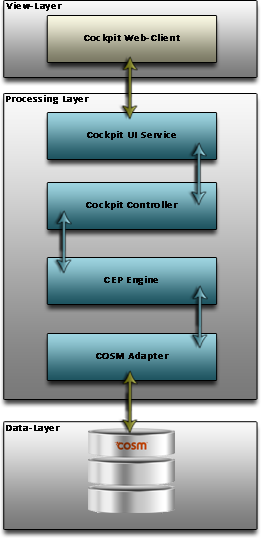
\includegraphics[scale=0.5]{Component-Overview.png}
		\caption[Angiogenetic Switch]{Angiogenetic Switch}
		\label{fig:AngiogeneticSwitch}
	\end{center}
\end{figure}

This component is a processing unit that is programmed with rules that results again in events. This rules are designed for the special use case of our cockpit. It forms one or many events in a temporal context to complex events that also can be the source for new rules. It is a detection for events that could be a derivation for complex events and so we adding new more valuable events than the simple events could do.
This (complex) events are used by the third component that registered as listener.
This component contains the business model. The model is updated with every event the component receives. 
To visualize this data we are providing the information as a service via a websocket api.
Our javascript client act as visualization unit that could connect to the service component and receive updates via websocket every time a state-change happens at then model site.
Through this chain of event-processing also the client receives the events triggered by the COSM-API in real-time and can provide this information for multiple clients.





\begin{itemize}
	\item EDA
	\item loose coupled components
	\item Add more event sources
	\item supply more processing units
	\item event driven architecture is extremely loosely coupled and well distributed
	\item communication via events
	\item even the source from other service is pushed via events
	\item 3 components
	\item COSM, ESPER, JS FrontEnd
	\item cosm
	\item websocket protokol
	\item cosm API
	\item transformation
	\item internal event structure
	\item 
\end{itemize}


On the conceptual level we have three different components that handle this job.
At first there is a connector that receive data from the COSM Service via the WebSocket-Protocol. The COSM Services Pushes Data via an defined API and the component forms that messages into Events into our EDA.

\section{Implementation}
\label{sec:Implementation}

\begin{itemize}
	\item Introduction
	\item Diagrams
	\item Real-Time event monitoring
	\item Short Desc
	\item Backend in Java
	\item Build with Maven
	\item Tomcat Maven Plugin to easy run
	\begin{itemize}
		\item COSM
		\item Route Model as COSM Sensors
		\item Implementation COSM
		\begin{itemize}
			\item Java
			\item COSMWebSocketEngine
			\item Simple Interface
			\item start,stop,listener
			\item AsyncHttpClient
			\item Websocket Protokol
			\item API
			\item API Key
			\item Response, HTTP Resp Wrapper 
			\item http docs beta socket server 
			\item SUBSCRIBE to DataStream
			\item unsuscribe for closing
			\item Objekt Parsing
			\item mapped to events
			\item Push To Esper via Listener Interface
		\end{itemize}
		\item Esper
		\begin{itemize}
			\item General Concept
			\item Complex Events
			\item Rules
			\item Listeners
			\item alternative Siddhi
		\end{itemize}
		\item JS Frontend
		\begin{itemize}
			\item Websocket Event Model
			\item Short Desc Components
			\item Google Maps Route
			\item jQuery Table visualization
		\end{itemize}
	\end{itemize}
\end{itemize}


\section{Conclusion}
\label{sec:Conclusion}
\begin{itemize}
	\item FI
	\item State-of-the art technologies
	\item real time events
	\item Logistic Information System / Business Process Management
	\item Multi-Device Support HTML5
\end{itemize}
%\end{document}  % This is where a 'short' article might terminate

%
% The following two commands are all you need in the
% initial runs of your .tex file to
% produce the bibliography for the citations in your paper.
\bibliographystyle{abbrv}
\bibliography{sigproc}  % sigproc.bib is the name of the Bibliography in this case
% You must have a proper ".bib" file
%  and remember to run:
% latex bibtex latex latex
% to resolve all references
%
% ACM needs 'a single self-contained file'!
%
%APPENDICES are optional
%\balancecolumns
\appendix
%Appendix A
\end{document}
